%
% Copyright (c) 2020 Antonio Coín Castro
%
% This work is licensed under a
% Creative Commons Attribution-ShareAlike 4.0 International License.
%
% You should have received a copy of the license along with this
% work. If not, see <http://creativecommons.org/licenses/by-sa/4.0/>.

In this last chapter we will present, study and provide a general method to solve some classic implicit equations. These equations were first proposed in the 18th and 19th centuries by renowned mathematicians of the time, and have since been deeply studied. We feel it is illustrative to discuss them here and bring this exposition to an end with some relevant and non-trivial examples. We will try to provide a variety of perspectives into these equations, and apply when possible the techniques that we have studied throughout this work.

\section{Clairaut equation}

We begin with the study of an implicit differential equation introduced by French mathematician A. Clairaut in 1734, which appears in geometric problems in which it is required to determine a curve in terms of a prescribed property of its tangents at all points, as we will shortly verify. A Clairaut equation takes the form
\begin{equation}  \label{eq:clairaut}
  y=xy' + f(y'),
\end{equation}
where $f$ is a continuously differentiable function. Clairaut was the first to point out the differences between the general and singular solutions of equations of this type, and this is why they bear his name. Since then, this equation has taken an important place in the theory of implicit equations; it has been generalized to higher dimensions and it has even been proposed as a model for a family of implicit equations with particular properties (see \cite{dara1975singularites}).

There are a number of ways to tackle this equation, ranging from an exhaustive theoretical study to a fast substitution method that works in practice. They all produce the same solutions, but the interpretation of the solving process is what changes among them. First we start with the geometrical approach. If we define $F(x,y,p)=y-xp -f(p)$ and revisit the theory developed in Chapter $\ref{ch:implicit}$, we should be able to write the equations of the surface $M=F^{-1}(0)$ and of the tangent and contact planes associated,
\[
  \begin{cases}
    y-xp-f(p)=0,\\
    p\,dx - dy -x\,dp -f'(p)\,dp=0,\\
    dy=p\,dx.
  \end{cases}
\]
Now, from the second and third equations we get the relation
\begin{equation} \label{eq:clairaut1}
(x+f'(p))\,dp = 0.
\end{equation}
On the other hand, we have $F_p = -(x+f'(p))$, so the criminant is composed by the points on $M$ for which $x=-f'(p)$. Outside of those points, equation \eqref{eq:clairaut1} implies that the integral curves on $M$ are the lines $p=C$, and when projected on the $(x,y)$-plane (substituting $p=C$ in the expression of $F$) we get the family of lines
\begin{equation} \label{eq:clairaut-general}
y=xC + f(C),
\end{equation}
 which is the general solution of the equation. Thus we can say that \textit{a Clairaut equation is the equation of a family of lines parametrized by the slope}.

Turning our attention towards the points on the criminant, we note that they are all improper singular points, since $F_x+pF_y=0$ holds everywhere. We can project these singular points and get the expression for the discriminant curve in parametric form as
\begin{equation} \label{eq:clairaut-singular}
x=-f'(p), \quad y = -pf'(p) + f(p),
\end{equation}
where $p$ is now the parameter along the curve. This singular solution turns out to be the envelope of the family \eqref{eq:clairaut-general} of straight lines with arbitrary slope, say $p$. Indeed, a quick calculation of the tangent at each point of the singular curve yields

\[
\frac{dy}{dx} = \frac{dy/dp}{dx/dp} = \frac{-f'(p)-pf''(p)+f'(p)}{-f''(p)}=p,
\]
given that $f''\neq 0$ at the point of interest. It can also be checked that curves consisting on arbitrary segments of the singular solution and the two lines of the family \eqref{eq:clairaut-general} tangent to it at each end of the segment are solutions of the equation as well, including the degenerate case in which the segment is a single point. In other words, infinitely many solutions of the equation pass through each point of the envelope.

Another method for solving this equation more directly but arguably losing the intuition behind it is to consider the original expression $y-xy'-f(y')=0$, introduce a parameter $p=dy/dx$ and differentiate with respect to $x$, obtaining
\[
p-p-xp'-f'(p)p' =0 \implies -(x+f'(p))p' =0.
\]
Now either $p'=0$ or $x+f'(p)=0$. In the first case we have $p=y'=C$, and substituting back in \eqref{eq:clairaut} one gets the general solution $y=xC+f(C)$. In the second case proceeding as before we can express the result in the same parametric form as in \eqref{eq:clairaut-singular}.

\begin{example} We will now analyze the Clairaut equations with $f(p)=p^2$ and $f(p)=p^3$. For the first case the lines $y=xp+p^2$, $p \in \R$ constitute the family of general solutions, while the curve
  \[
x=-2p,\quad y = -p^2,\quad p \in \R
  \]
is the singular solution, which can also be written explicitly eliminating the parameter as $y=\frac{-x^2}{4}$. The general and singular solutions are shown in Figure \ref{fig:clairaut-sol1}.

\begin{figure}[h!]
\centering
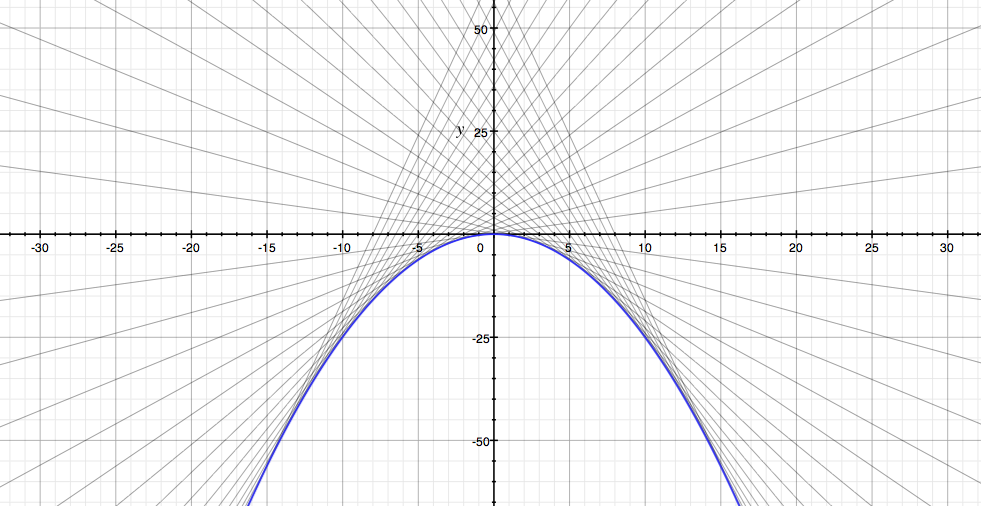
\includegraphics[width=.65\textwidth]{clairaut1}
\caption{Representation\protect\footnotemark  of the solutions of the equation $y=xy'+(y')^2$.}
\label{fig:clairaut-sol1}
\end{figure}

\footnotetext{%
Both this figure and the next one were created by Alex Hall and are \href{https://en.wikipedia.org/wiki/File:Solutions_to_Clairaut\%27s_equation_where_f(t)\%3Dt\%5E2.png}{freely} \href{https://en.wikipedia.org/wiki/File:Solutions_to_Clairaut\%27s_equation_where_f(t)\%3Dt\%5E3.png}{distributed} on Wikimedia Commons under a CC-BY-SA 3.0 license.
}%

We can see from Figure \ref{fig:clairaut-sol1} that if we choose a point $(x_0,y_0)$ under the singular curve, there is no solution passing through this point. On the other hand, we observe that the singular parabola and the line $y=xp+p^2$ intercept at the point $(-2p,-p^2)$, so for example the curves
\[
\phi_p(x)= \begin{cases}
  xp + p^2, & x < -2p,\\
  \frac{\displaystyle -x^2}{\displaystyle 4} & x \ge -2p
\end{cases}
\]
are also solutions of the equation for every choice of $p\in \R$.

In a completely analogous way, the general solution of $y=xy'+(y')^3$ is the family of lines $y=xp+p^3$, $p\in\R$, and the singular solution is the curve given implicitly by the equation
\[
y^2=\frac{-4x^3}{27}, \quad x \le 0,
\]
as shown in Figure \ref{fig:clairaut-sol2}. Unlike the previous example, in this case there is at least one solution passing through every point of the $(x,y)$-plane.

\begin{figure}[h!]
\centering
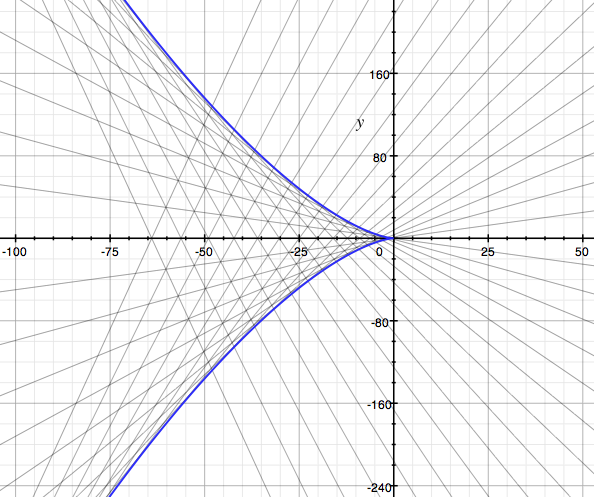
\includegraphics[width=.55\textwidth]{clairaut2}
\caption{Representation of the solutions of the equation $y=xy'+(y')^3$.}
\label{fig:clairaut-sol2}
\end{figure}

\end{example}

\section{Lagrange equation}

The next equation we consider is the family of Lagrange equations,
\begin{equation}\label{eq:lagrange}
  y=xf(y')+g(y'),
\end{equation}
where both $f$ and $g$ are defined and continuously differentiable in some open interval $I\subset \R$. These equations are named after Joseph Louis Lagrange\footnote{They are also associated with d'Alembert, so in some texts they are referred to as d'Alembert equations.}, who also studied the theory of implicit differential equations and singular solutions in the second half of the 18th century, and discussed this specific equation in \cite{lagrange1759integration}. One thing to note from the start is that when $f$ is the identity function, equation \eqref{eq:lagrange} reduces to a Clairaut equation, so in some sense this new equation is a generalization of the former.

To solve this equation the most straightforward method is to introduce the parameter $p=dy/dx$ and differentiate the equation with respect to $x$, obtaining
\begin{equation} \label{eq:lagrange1}
  p=f(p)+xf'(p)p' + g'(p)p' \implies p-f(p) = (xf'(p)+g'(p))p'.
\end{equation}
Now we consider firstly the case when $p'=0$, that is, $p=y'=C \in I$. Equation \eqref{eq:lagrange1} implies that $p=f(p)$, and substituting this information back into \eqref{eq:lagrange} gives us that the straight line $y=xC+g(C)$ is a solution of the equation. Thus, the family
\[
\left\{y=xC+g(C): C \text{ is a root of } p-f(p) = 0\right\}
\]
is a family of solutions of the equation, which might or might not be singular. It can also be shown that these are the only straight lines that are solutions of the equation.

Assuming that $p\neq f(p)$, equation \eqref{eq:lagrange1} implies that $dp/dx\neq 0$, and then we can apply the inverse function theorem to write $x=x(p)$. In this case, equation \eqref{eq:lagrange1} reads
\begin{equation}\label{eq:lagrance-linear}
  \frac{dx}{dp} = \frac{xf'(p)+g'(p)}{p-f(p)}.
\end{equation}
This is a linear differential equation in the independent variable $p$, which will have a general solution, say $x=\Phi(p,C)$. Substituting back into the original equation, we have found the family of general solutions of equation \eqref{eq:lagrange}, which is expressed as a function of the parameter $p$ as
\[
x=\Phi(p,C),\quad y=\Phi(p,C)f(p) + g(p).
\]

\begin{example} Let us consider the Lagrange equation
  \begin{equation}\label{eq:lagrange-ex}
    y=2xy'-(y')^2.
  \end{equation}

We identify the functions $f(p)=2p$ and $g(p)=-p^2$. Solving $f(p)=p$ for $p$ yields $p=0$, so the only solution line is that of slope $0$ passing through the point $(0,g(0))=(0,0)$, that is, the horizontal line $y=0$. If we analyzed the criminant of this equation, we would realize that it is composed of the points on the solution surface for which $x=p$, so the line $y=0$ is not a singular solution of the equation.

If $p'\neq 0$, setting $y'=p$ in the equation and differentiating with respect to $x$ yields
\[
-p=p'(2x-2p),
\]
which since $p'\neq 0$ we can rewrite as the linear ODE
\[
\frac{dx}{dp}= \frac{-2}{p}x + 2.
\]
This equation gives the general solution $x(p)=\frac{2}{3}p+\frac{C}{p^2}$, which we can substitute in our equation to get the family of general solutions of \eqref{eq:lagrange-ex}, depicted in Figure \ref{fig:lagrange}:
\[
\begin{cases}
  \displaystyle x=\frac{2}{3}p+\frac{C}{p^2},\\
  \displaystyle y=\frac{1}{3}p^2+\frac{2C}{p},
\end{cases}\quad p \neq 0.
\]

\begin{figure}[h!]
\centering
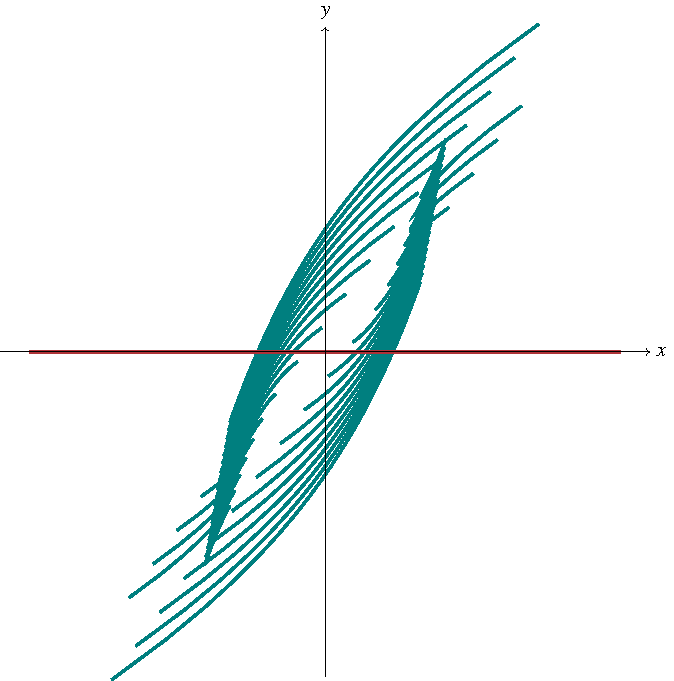
\includegraphics[width=.6\textwidth]{lagrange}
\caption{Representation of the family of solutions of the equation $y=2xy'-(y')^2$.}
\label{fig:lagrange}
\end{figure}

\end{example}

\section{Chrystal equation}

Lastly we present an equation studied at the end of the $19$th century by G. Chrystal, who took a closer look at its potential singular solutions (see \cite{chrystal1897discriminant} for the original article). A Chrystal equation assumes the form
\begin{equation} \label{eq:chrystal}
  (y')^2 + Axy' + By + Cx^2=0,
\end{equation}
where $A,B,C$ are real-valued constants. As we will see below, under certain conditions this equation is yet another generalization of the Clairaut equation, which stresses the importance of the latter in the theory of implicit equations throughout the modern history of mathematics. The Chrystal equation is discussed in some detail in \cite{ince1956ordinary} and \cite{davis1962introduction}.

The solving process for this equation begins by solving \eqref{eq:chrystal} for $y'$ and considering at the same time the two resulting differential equations, that is,
\begin{equation}\label{eq:chrystal1}
  y' = -\frac{A}{2}x \pm \frac{1}{2}(A^2x^2-4By-4Cx^2)^{1/2}.
\end{equation}
Now we introduce a new variable $z=z(x)$ by means of the relation
\begin{equation} \label{eq:chrystal5}
  4By=(A^2-4C-z^2)x^2,
\end{equation}
so that equation \eqref{eq:chrystal1} reduces to
\[
xzz'=A^2+AB -4C - z^2 \pm Bz.
\]
This equation is separable and can be written as
\begin{equation}\label{eq:chrystal2}
  \frac{dx}{x} = \frac{z\,dz}{A^2+AB -4C - z^2 \pm Bz}.
\end{equation}

The next step is to factorize the denominator in the right hand side of \eqref{eq:chrystal2}. If we denote by $a$ and $b$ the two combined roots of the equation
\begin{equation} \label{eq:chrystal3}
  A^2+AB -4C - z^2 \pm Bz =0,
\end{equation}
we can rewrite equation \eqref{eq:chrystal2} in the form
\begin{equation} \label{eq:chrystal4}
\frac{dx}{x}=\frac{z\,dz}{(z-a)(z-b)}.
\end{equation}
It can be proven (via direct integration) that if $a\neq b$, the solutions of this equation take the form
\[
x\dfrac{(z-a)^{a/(a-b)}}{(z-b)^{b/(a-b)}} = k, \quad k \in \R,
\]
and if $a=b$ then the solutions\footnote{A more profound analysis of the transcendental solutions that arise in this case can be found in \cite{jordan2010note}.} are
\[
x(z-a)\exp \left( \frac{a}{a-z} \right) = k, \quad k \in \R.
\]
In each case we can substitute back into \eqref{eq:chrystal5} using these expressions, and hence we get the solutions to our equation in parametric form, where now $z$ is the parameter.

Apart from this general procedure, the case when one of the roots $a$ or $b$ is $0$ merits special attention. Suppose without loss of generality that $a=0$. Then by equation \eqref{eq:chrystal3} we have
\begin{equation} \label{eq:chrystal6}
  A^2+AB -4C=0,
\end{equation}
so the other root is $b=\pm B$, which we will suppose is non-zero for the sake of the argument. In this case the solutions to \eqref{eq:chrystal4} are expressed as
\[
x(z\pm B) = k, \quad k \in \R,
\]
and then we assert that the solutions of \eqref{eq:chrystal} are recovered as
\begin{equation} \label{eq:chrystal-parabola}
  4By = -ABx^2 - (k \pm Bx)^2, \quad k \in \R.
\end{equation}
To see this, note that from $x(z\pm B)=k$ we get $xz=k\pm Bx$, and substituting this expression into \eqref{eq:chrystal5} yields
\[
4By=x^2(A^2-4C)-(k\pm Bx)^2.
\]
Finally, equation \eqref{eq:chrystal6} allows us to write $A^2-4C=-AB$, arriving at the desired result.

It is worth pointing out that the family of parabolas we get as solutions in this case has an envelope, namely
\[
y= -\frac{A}{4}x^2.
\]
This expression can be derived employing the usual techniques, and it can be seen that this parabola is tangent to the family \eqref{eq:chrystal-parabola} at each point, so it is indeed its envelope. In other words, when condition \eqref{eq:chrystal6} holds we have a singular solution of the equation. If we take a closer look at the process this fact should not come as a surprise, since under the conditions mentioned equation \eqref{eq:chrystal5} reduces to the Clairaut form.
